% !TeX root = ../thesis.tex
\فصل{روش پژوهش و راهکار پیشنهادی}

در این فصل، مراحل آماده‌سازی داده‌ها، آموزش مدل‌ها و طراحی آزمایش‌ها تشریح می‌شود. آزمایش‌ها به‌گونه‌ای طراحی شده‌اند که بتوان اثر روش‌های مختلف را جدا از یکدیگر بررسی کرد. از یک سو، هدف افزایش مقاومت بازشناس در برابر شرایط تلفنی و صدا بر بستر پروتکل اینترنت\پاورقی{Voice over IP (VoIP)} است و از سوی دیگر، استفاده از گفتار بدون رونویسی به‌عنوان راهی برای افزایش حجم و تنوع داده‌های آموزشی بررسی می‌شود. به همین دلیل، در هر آزمایش تنها عامل مورد نظر تغییر داده شده و سایر اجزای آموزش و ارزیابی تا حد ممکن یکسان نگه داشته شده‌اند.

آزمایش‌های اصلی در دو محور و با چهار پیکربندی ویسپر-کوچک انجام شدند. در محور نخست، مقاومت مدل در شرایط مخابراتی بررسی شد. برای این منظور، یک مدل با داده‌های معمولی فارسی و مدل دیگر با ترکیبی از داده‌های معمولی و نسخه‌های مصنوعی تخریب‌شده آن‌ها ریزتنظیم شدند. سپس مدل دوجریانه همجوشی با استفاده از داده‌های تخریب‌شده آموزش داده شد. در محور دوم، تأثیر افزایش حجم داده بررسی شد؛ به این منظور، همان داده‌های آموزش چندشرایطی حفظ شد و گفتار شبه‌برچسب‌خوردهٔ ایران‌صدا به آن افزوده شد. در کنار این آزمایش‌ها، دو بررسی تکمیلی نیز انجام شد: فست کانفورمر برای سنجش اثر آموزش چندشرایطی در خانواده‌ای متفاوت از مدل‌های بازشناسی، و ویسپر-متوسط\پاورقی{Whisper Medium} که هم به‌عنوان معلم تولید شبه‌برچسب و هم به‌عنوان مدلی با ظرفیت بیشتر ارزیابی شد.

\قسمت{طراحی پژوهش و زنجیرهٔ مقایسه‌ها}

با توجه به پرسش‌های پژوهش که در فصل مقدمه مطرح شده‌اند، جدول~\رجوع{جدول:طرح-مقایسه‌ها} طراحی آزمایش را در سه مقایسه مستقیم خلاصه می‌کند و عامل متغیر و حدود تفسیر هر مقایسه را نشان می‌دهد. 


\شروع{لوح}[htbp]
\تنظیم‌ازوسط
\شرح{طرح مقایسه‌ای مسیرهای اصلی پژوهش}
\resizebox{\textwidth}{!}{%
\شروع{جدول}{|p{0.15\textwidth}|p{0.25\textwidth}|p{0.22\textwidth}|p{0.30\textwidth}|}
\خط‌پر
\سیاه مسیر & \سیاه مقایسهٔ مستقیم & \سیاه عامل ثابت & \سیاه دامنهٔ تفسیر \\
\خط‌پر \خط‌پر
مقاوم‌سازی داده‌محور & ویسپر معمولی در برابر ویسپر چندشرایطی & معماری، مدت آموزش، نرخ یادگیری و قواعد ارزیابی & اثر افزودن داده تخریب‌شده در پیکربندی اجراشده \\
\خط‌پر
مقاوم‌سازی مدل‌محور & ویسپر چندشرایطی در برابر مدل دوجریانه & نقطهٔ آغاز چندشرایطی، روش تخریب و مجموعه‌های آزمون & اثر سامانه کامل بهسازی-همجوشی \\
\خط‌پر
افزایش مقیاس داده & ویسپر چندشرایطی در برابر ویسپر چندشرایطی همراه با ایران‌صدا & معماری ویسپر-کوچک، تنظیمات اصلی آموزش، داده‌های پیشین و ارزیابی & اثر افزودن پیکره شبه‌برچسب‌خورده \\
\خط‌پر
\پایان{جدول}}
\برچسب{جدول:طرح-مقایسه‌ها}
\پایان{لوح}

\قسمت{داده‌ها و پیش‌پردازش}

\زیرقسمت{داده‌های آموزش و اعتبارسنجی}

پیکرهٔ پایه آموزش این پژوهش از کامن‌وویس فارسی نسخه $25$\پاورقی{Common Voice Persian 25}، فلورز فارسی\پاورقی{FLEURS Persian} و پیکره فارس‌اسپان\پاورقی{FarsSpon} تشکیل شده است. این پیکره‌ها از نظر نوع گفتار و دامنه مکمل یکدیگرند؛ کامن‌وویس تنوع بالایی از گویندگان را در بر می‌گیرد، فلورز شامل گفتار خوانده‌شده از حوزه‌های متفاوت است و فارس‌اسپان گفتار بداهه فارسی را پوشش می‌دهد \مرجع{commonvoice2024,conneau2022fleurs}. داده ایران‌صدا نیز جدا از این مجموعه نگه داشته شد و فقط در آزمایش مربوط به افزایش حجم داده به مجموعه آموزش اضافه شد.

پیش از استفاده از این داده‌ها برای آموزش، همه فایل‌های صوتی به صوت تک‌کاناله با نرخ نمونه‌برداری $16$ کیلوهرتز تبدیل شدند. رونویسی‌ها نیز با یک نرمال‌ساز فارسی پردازش شدند تا تفاوت‌های نوشتاری مربوط به شکل حروف «ی» و «ک»، فاصله و نیم‌فاصله، نشانه‌گذاری و نمایش اعداد کاهش یابد. این نرمال‌سازی روی متن آموزش، متن مرجع و خروجی مدل نیز اعمال شد تا تفاوت‌های نوشتاری بر محاسبه معیارهای ارزیابی اثر نگذارند.

\شروع{لوح}[ht]
\تنظیم‌ازوسط
\شرح{مجموعه‌داده‌های پایه آموزش و اعتبارسنجی پیش از افزودن ایران‌صدا}
\شروع{جدول}{|c|c|c|c|}
\خط‌پر
\سیاه مجموعه‌داده & \سیاه تعداد آموزش & \سیاه تعداد اعتبارسنجی & \سیاه نقش در آزمایش \\
\خط‌پر \خط‌پر
کامن‌وویس فارسی ۲۵ & \lr{299,430} & \lr{10,006} & آموزش عمومی و تولید داده تخریب‌شده \\
فارس‌اسپان (محدود) & \lr{600,672} & \lr{6,044} & آموزش گفتار بداهه فارسی \\
فلورز فارسی & \lr{3,019} & \lr{362} & آموزش و افزایش تنوع دامنه \\
\خط‌پر
\پایان{جدول}
\برچسب{جدول:داده-آموزش}
\پایان{لوح}

از آنجا که بخش زیادی از نمونه‌های کامن‌وویس و فارس‌اسپان کوتاه هستند، نسخه‌هایی با قطعه‌های بلندتر نیز از این دو پیکره ساخته شد تا مدل در زمان آموزش با توالی‌های گفتاری طولانی‌تری روبه‌رو شود. برای ساخت هر نمونه، دو تا چهار کلیپ از یک بخش داده به یکدیگر متصل شدند؛ به‌گونه‌ای که طول نهایی بیش از $5$ و حداکثر $20$ ثانیه باشد. رونویسی کلیپ‌ها نیز به همان ترتیب با یکدیگر ترکیب شد. این نمونه‌ها که در ادامه «گونه‌های بلند» نامیده می‌شوند، در آموزش تمام مدل‌های اشاره شده در قسمت‌های بعد استفاده شدند. در آموزش چندشرایطی، علاوه بر داده‌های اصلی، از هر کلیپ کامن‌وویس و گونه بلند آن دو نسخهٔ تخریب‌شده مستقل با همان رونویسی تولید شد.

\زیرقسمت{مجموعه‌های آزمون}

ارزیابی روی پنج مجموعه مستقل از داده‌های اعتبارسنجی انجام شد. چهار مجموعه داده، عملکرد مدل را در دامنه‌های عمومی فارسی سنجیدند و داده AGFarsdat برای ارزیابی عملکرد مدل روی گفتار تلفنی استفاده شد.


مجموعهٔ خصوصی \مهم{AGFarsdat} شامل گفتار واقعی تلفنی و \lr{VoIP} است و با شبیه‌ساز این پژوهش ساخته نشده است. این مجموعه ۱۰۰۴۴ گفتهٔ رونویسی‌شده از ۵۸۵ گوینده و ۴۹٫۹ ساعت صوت تک‌کانالهٔ ۸ کیلوهرتز و ۱۶ بیت دارد. بازنشر آن مجاز نیست و اطلاعات کامل شیوه گردآوری، ویژگی‌های جمعیت‌شناختی گویندگان، رضایت و مجوز در دسترس قرار نگرفته است. این محدودیت‌ها دامنه تحلیل مجموعه را کاهش می‌دهند، اما از نقش آن به‌عنوان آزمون نهایی مخابراتی نمی‌کاهند.


مجموعه‌های دیگر دامنه‌های عمومی‌تر فارسی را پوشش می‌دهند و مشخص می‌کنند که مقاوم‌سازی مخابراتی چه اثری بر گفتار غیرمخابراتی دارد. پرشین‌اسپیچ از مجموعه عمومی منتشرشده در مخزن \کد{persiandataset/PersianSpeech} آماده شد \مرجع{persianspeech2026}. «پیکرهٔ گفتار فارسی» نیز پیکره‌ای عمومی و تک‌گوینده است که با لهجه تهرانی و در محیط استودیویی ضبط شده است \مرجع{halabiPersianSpeechCorpus}. جدول~\رجوع{جدول:داده-آزمون} اندازه و نقش هر مجموعه را نشان می‌دهد.

\شروع{لوح}[ht]
\تنظیم‌ازوسط
\شرح{مجموعه‌های ارزیابی و نقش آن‌ها}
\شروع{جدول}{|c|c|c|}
\خط‌پر
\سیاه مجموعه & \سیاه تعداد نمونهٔ ارزیابی‌شده & \سیاه ویژگی و نقش \\
\خط‌پر \خط‌پر
AGFarsdat & \lr{10,044} & ۵۸۵ گوینده و ۴۹٫۹ ساعت؛ آزمون نهایی مخابراتی \\
کامن‌وویس فارسی ۲۵ & حدود \lr{10,518} & گفتار عمومی برون‌سپاری‌شده \\
فلورز فارسی & \lr{871} & گفتار خوانده‌شده چنددامنه \\
پرشین‌اسپیچ & \lr{24} & مجموعهٔ آزمون فارسی با حجم کم \\
پیکرهٔ گفتار فارسی & \lr{391--396} & گفتار فارسیِ برون‌دامنه \\
\خط‌پر
\پایان{جدول}
\برچسب{جدول:داده-آزمون}
\پایان{لوح}


\قسمت{تولید دادهٔ مخابراتی مصنوعی}

\زیرقسمت{ساخت جفت‌های پاک-تخریب‌شده}

به‌دلیل محدودبودن گفتار تلفنی واقعیِ رونویسی‌شده و تفاوت شرایط آن با داده‌های آموزشی، از گفتار آموزشی جفت‌های هم‌تراز پاک-تخریب‌شده ساخته می‌شوند. هر جفت رونویسی یکسانی دارد: نسخه تخریب‌شده به‌عنوان ورودی بازشناس و نسخه پاکِ هم‌پهنای‌باند به‌عنوان هدف آموزش ماژول بهساز در مدل همجوشی استفاده می‌شود. در ماژول بهساز هدف به تولید صوت پاک هم‌پهنای‌باند با نسخه تخریب‌شده محدود می‌شود تا بهساز برای بازسازی مؤلفه‌های فرکانسی‌ای که در اثر محدودیت کانال حذف شده‌اند جریمه نشود و آموزش آن بر کاهش نویز و اعوجاج‌های ایجادشده در محدوده قابل مشاهده متمرکز بماند. 

\زیرقسمت{نمایه‌های تخریب}

برای تولید هر نمونه، ابتدا یکی از چهار نمایه (پروفایل) مندرج در جدول~\رجوع{جدول:نمایه-تخریب} انتخاب می‌شود. منظور از نمایه، مجموعه‌ای از تنظیمات و احتمالات است که مشخص می‌کند کدام تخریب‌ها و با چه احتمالی روی نمونه موردنظر اعمال شوند. به‌کارگیری هر نمایه به ایجاد سناریوهای متنوع مخابراتی کمک می‌کند؛ برای نمونه، یک نمایه می‌تواند شرایط یک تماس تلفنی باریک‌باند همراه با نویز بالا را شبیه‌سازی کند، درحالی‌که نمایه دیگر بر شرایط تماس \lr{VoIP} و افت بسته‌ها تمرکز دارد. بنابراین، نمایه خود یک نوع تخریب مجزا نیست، بلکه چارچوبی است برای نمونه‌برداری تصادفی از نویز، کدک، پهنای‌باند و اختلالات شبکه.

احتمال‌ها و وزن‌های این نمایه‌ها با هدف ایجاد تنوع در داده آموزشی و پوشش شرایط مخابراتی مختلف انتخاب شدند؛ به‌گونه‌ای که هم نمونه‌های نسبتاً پاک و هم شرایط دشوارتر مانند نویز و افت بسته به تعداد کافی در آموزش حضور داشته باشند. برای نمونه، احتمال اختلال شبکه در نمایه \lr{VoIP} افت‌ بسته بیشتر در نظر گرفته شده، زیرا هدف اصلی این نمایه بازنمایی همین نوع تخریب است. این مقادیر از آمار یک اپراتور یا اندازه‌گیری تماس‌های واقعی استخراج نشده‌اند و تنها توزیع طراحی‌شده برای ساخت داده آموزشی را مشخص می‌کنند. 

\شروع{لوح}[ht]
\تنظیم‌ازوسط
\شرح{نمایه‌های تخریب در پیکربندی اجراشده}
\resizebox{\textwidth}{!}{%
\شروع{جدول}{|c|c|c|c|}
\خط‌پر
\سیاه نمایه & \سیاه وزن انتخاب & \سیاه احتمال نویز & \سیاه مسیر غالب \\
\خط‌پر \خط‌پر
\کد{telephone\_clean} & \lr{0.25} & \lr{0} & باریک‌باند: G.711 A-law/$\mu$-law، GSM، AMR-NB \\
\کد{telephone\_noisy} & \lr{0.30} & \lr{0.70} & باریک‌باند: G.711 A-law/$\mu$-law، GSM، AMR-NB \\
\کد{voip\_lossy} & \lr{0.25} & \lr{0.30} & Opus پهن‌باند/باریک‌باند با افت بسته و PLC \\
\کد{mobile\_wideband} & \lr{0.20} & \lr{0.45} & AMR-WB، Opus پهن‌باند یا عبور مستقیم \\
\خط‌پر
\پایان{جدول}}
\برچسب{جدول:نمایه-تخریب}
\پایان{لوح}

در نمایه‌هایی که افزودن نویز فعال است، یک نمونه از مجموعه نویز دیمند\پاورقی{DEMAND} با گفتار ترکیب می‌شود و با احتمال $0.10$ نمونه نویز دیگری نیز به آن افزوده می‌شود \مرجع{thiemann2013demand}. نویز متناسب با طول گفتار بریده یا تکرار می‌شود و پیش از تغییر بهره و اعمال کدک به سیگنال اضافه می‌شود. نسبت سیگنال به نویز از یکی از چهار بازهٔ $[10,15]$، $[5,10]$، $[0,5]$ و $[-5,0]$ دسی‌بل و تغییر بهره از بازهٔ $[-6,+6]$ دسی‌بل نمونه‌برداری می‌شود. بازه‌های انتخاب‌شده شرایطی از نویز نسبتاً ضعیف تا حالتی را پوشش می‌دهند که توان نویز از گفتار بیشتر است. تغییر بهره نیز پس از اختلاط روی کل سیگنال اعمال می‌شود؛ بنابراین، گفتار و نویز به یک نسبت مقیاس می‌شوند و نسبت سیگنال به نویز تغییر نمی‌کند. در نمایه \lr{telephone\_noisy}، علاوه بر احتمال بیشتر افزودن نویز، احتمال اعمال اختلال شبکه نیز دو برابر \lr{telephone\_clean} در نظر گرفته شده است تا این نمایه شرایط دشوارتری از تماس تلفنی را بازنمایی کند.


\زیرقسمت{زنجیره کانال، کدک و اختلال شبکه}

ترتیب کلی مراحل در شکل~\رجوع{شکل:معماری-خط-لوله-تخریب} نشان داده شده است. ابتدا نویز به گفتار افزوده می‌شود، سپس محدودیت پهنای‌باند و کدک اعمال می‌شوند و در صورت فعال‌بودن اختلال شبکه، افت بسته در شاخه مربوط شبیه‌سازی می‌شود. علاوه بر این تخریب‌ها، کنترل دامنه، جبران تأخیر، هم‌ترازسازی طول و مقیاس‌دهی مشترک دو عضو جفت انجام می‌شود تا اختلاف‌های ناخواسته‌ای که مستقیماً به شرایط مخابراتی مربوط نیستند وارد داده نشوند.


\شروع{شکل}[htbp]
\centering
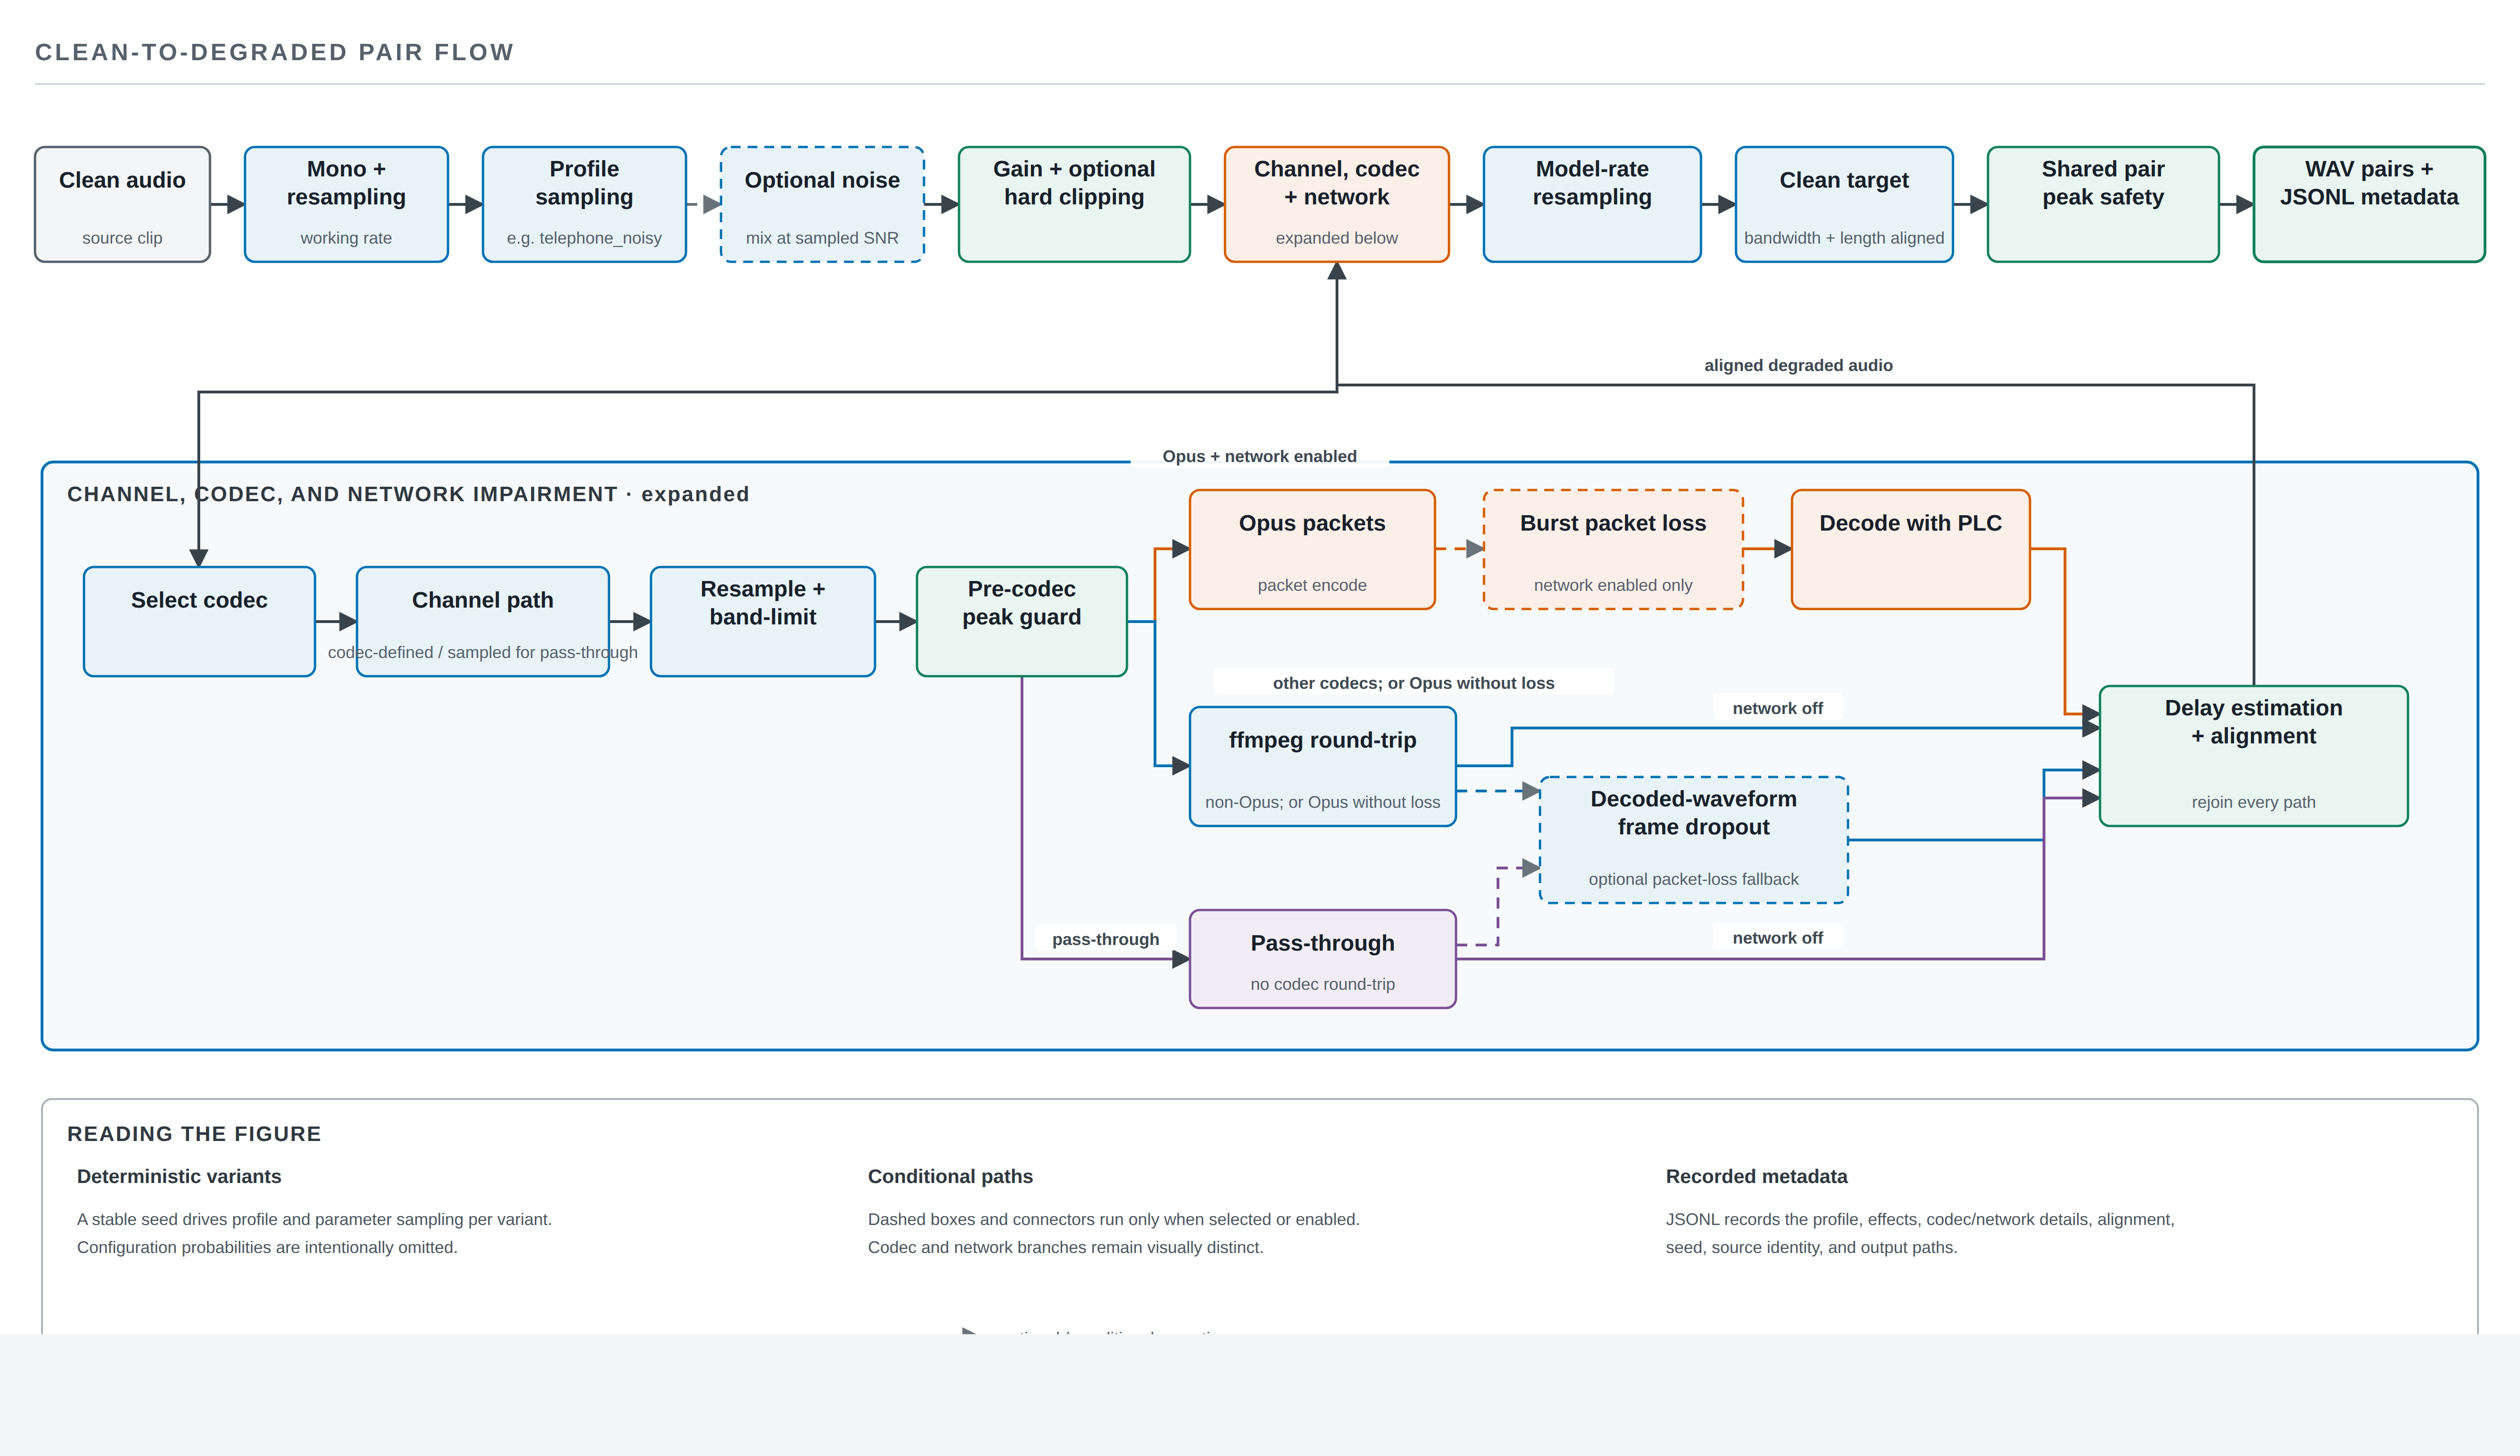
\includegraphics[width=\linewidth,height=0.62\textheight,keepaspectratio]{figs/degradation-pipeline-architecture.png}
\شرح{معماری خط لوله تولید جفت‌های پاک-تخریب‌شده. کادرها و یال‌های خط‌چین عملیات شرطی را نشان می‌دهند. انتخاب کدک مسیر باریک‌باند یا پهن‌باند را تعیین می‌کند.}
\برچسب{شکل:معماری-خط-لوله-تخریب}
\پایان{شکل}

مراحل این زنجیره به‌ترتیب عبارت‌اند از:

\شروع{فقرات}
\فقره بارگذاری صوت پاک، تبدیل به تک‌کاناله و بازنمونه‌برداری به نرخ کاری $16$ کیلوهرتز؛
\فقره انتخاب نمایه، اختلاط نویز و اعمال تغییر بهره؛
\فقره انتخاب مسیر باریک‌باند یا پهن‌باند و اعمال فیلتر کانال؛ در مسیر باریک‌باند، سیگنال با نرخ نمونه‌برداری $8$ کیلوهرتز و گذرباند تقریبی $300$ تا $3400$ هرتز پردازش می‌شود، درحالی‌که در مسیر پهن‌باند نرخ نمونه‌برداری $16$ کیلوهرتز و گذرباند تقریبی $50$ تا $7000$ هرتز در نظر گرفته می‌شود؛
\فقره کنترل بیشینه دامنه سیگنال پیش از تبدیل به \کد{PCM16}، به‌منظور جلوگیری از کلیپ‌شدن صوت و ورود سیگنال اعوجاج‌یافته به کدک؛
\فقره اجرای شاخهٔ کدک و شبکه. در مسیر Opus، اگر اختلال شبکه فعال باشد، بسته‌ها با مدل افت جهشی حذف می‌شوند و رمزگشا سازوکار PLC را به کار می‌گیرد. در کدک‌های دیگر، چرخه واقعی \کد{ffmpeg} اجرا می‌شود و اختلال شبکه با حذف قاب از موج رمزگشایی‌شده تقریب زده می‌شود. حالت عبور مستقیم کدک را کنار می‌گذارد، اما می‌تواند همین حذف قاب را دریافت کند. کدک‌های پشتیبانی‌شده عبارت‌اند از G.711 A-law، G.711 $\mu$-law، GSM، AMR-NB با نرخ $12.2$ کیلوبیت‌برثانیه، AMR-WB با نرخ $12.65$ کیلوبیت‌برثانیه و Opus باریک‌باند و پهن‌باند؛
\فقره برآورد و جبران تأخیر پس از پایان شاخه انتخاب‌شده، با هم‌بستگی متقاطع\پاورقی{cross-correlation} نسبت به موج پیش از کدک؛ و
\فقره بازنمونه‌برداری خروجی به $16$ کیلوهرتز، ساخت هدف پاکِ هم‌پهنای‌باند، هم‌ترازسازی طول و نرمال‌سازی جفت با مقیاس قلهٔ مشترک $0.99$.
\پایان{فقرات}

استفاده از چرخه واقعی رمزگذاری و رمزگشایی باعث می‌شود اعوجاج خود کدک نیز در سیگنال نهایی حضور داشته باشد. مسیر باریک‌باند محدودیت فرکانسی تلفن سنتی و برخی کدک‌های همراه را بازنمایی می‌کند، درحالی‌که مسیر پهن‌باند به تماس‌های جدیدتر مربوط است. خروجی هر دو مسیر در پایان به نرخ $16$ کیلوهرتز تبدیل می‌شود تا با قالب ورودی بازشناس یکسان بماند؛ بااین‌حال، این بازنمونه‌برداری اطلاعات فرکانسی حذف‌شده در مسیر باریک‌باند را بازیابی نمی‌کند.

در خط لوله تخریب، از چند کدک رایج مخابراتی شامل G.711، GSM، AMR و Opus استفاده می‌شود تا شرایط باریک‌باند و پهن‌باند تماس شبیه‌سازی شود \مرجع{itu1988g711,etsi2000gsm0610,3gpp2024amrnb,3gpp2024amrwb,valin2012opus}. رمزگذاری و رمزگشایی تا حد امکان با پیاده‌سازی واقعی کدک‌ها انجام می‌شود تا اعوجاج ایجادشده تنها به فیلترکردن یا کاهش مصنوعی کیفیت محدود نباشد. در حالت عبور مستقیم نیز چرخه کدک حذف می‌شود، اما محدودیت پهنای‌باند مسیر همچنان حفظ می‌شود.

اختلال شبکه با ایجاد افت‌های منفرد و پیاپی در بخشی از نمونه‌ها شبیه‌سازی می‌شود و احتمال و شدت آن به نمایه تخریب وابسته است. در مسیر Opus، افت در سطح بسته اعمال می‌شود و رمزگشا برای بخش‌های ازدست‌رفته از سازوکار پنهان‌سازی افت بسته\پاورقی{Packet-Loss Concealment (PLC)} استفاده می‌کند. برای سایر کدک‌ها، که چنین کنترلی در سطح بسته در دسترس نیست، اثر افت شبکه با حذف بخش‌هایی از موج رمزگشایی‌شده تقریب زده می‌شود \مرجع{ding2003assessment,fernandez2022augmentation}. بنابراین، شبیه‌سازی Opus به رفتار یک تماس \lr{VoIP} نزدیک‌تر است، درحالی‌که مسیر سایر کدک‌ها تنها تقریبی از اثر افت بسته را فراهم می‌کند.

پس از پایان این پردازش، تأخیر احتمالی ایجادشده در مسیر کدک جبران و طول دو عضو جفت یکسان می‌شود. برای ساخت هدف پاک نیز همان محدودیت پهنای‌باند مسیر تخریب‌شده روی گفتار اصلی اعمال می‌شود تا ماژول بهساز برای بازسازی مؤلفه‌های فرکانسی حذف‌شده جریمه نشود. در نهایت، هر دو موج با یک ضریب مشترک مقیاس می‌شوند تا رابطهٔ دامنه‌ای میان ورودی و هدف حفظ شود و از برش سیگنال جلوگیری شود.


این خط لوله شبیه‌ساز کامل تماس نیست. در نسخه حاضر، عواملی مانند پاسخ ضربه‌ای اتاق، پژواک، نوسان تأخیر و هم‌پوشانی گفتار چند گوینده مدل نشده‌اند و دامنه آزمایش به نویز محیطی، تغییر بهره، محدودیت پهنای‌باند، اعوجاج کدک و افت بسته محدود است و نتایج نیز باید با توجه به همین محدوده تفسیر شوند.

\قسمت{مدل‌های مبنای تک‌جریانه}

ویسپر-کوچک به‌دلیل توازن مناسب میان ظرفیت مدل و هزینهٔ محاسباتی، برای مقایسه‌های اصلی انتخاب شد \مرجع{radford2023robust}. در همهٔ آزمایش‌ها، صوت $16$ کیلوهرتزی به ویژگی‌های لاگ-مل $80$ بانده تبدیل شد و مدل با تنظیم زبان فارسی و حالت رونویسی اجرا شد و برای تابع زیان از آنتروپی متقاطع خودبازگشتی استفاده شد:

\begin{equation}
\mathcal{L}_{\mathrm{ASR}}=-\sum_{t=1}^{|\mathbf{y}|}
\log p_{\theta}\left(y_t\mid y_{<t},\mathbf{H}\right),
\end{equation}

که در آن $\mathbf{y}$ دنبالهٔ توکن‌های مرجع و $\mathbf{H}$ خروجی رمزگذار است.

دو مدل تک‌جریانه، هرکدام برای یک دوره و با نرخ یادگیری $10^{-5}$ آموزش داده شدند. اندازه دسته در هر دستگاه $4$ و تعداد گام‌های انباشت گرادیان $8$ بود؛ بنابراین، پیش از هر به‌روزرسانی وزن‌ها گرادیان $32$ نمونه تجمیع می‌شد. معماری، تنظیمات اصلی بهینه‌سازی و تعداد گام‌های آموزش در هر دو مدل یکسان بود و تفاوت اصلی میان آن‌ها به داده‌های مورد استفاده در آموزش مربوط می‌شد.

مدل معمولی با داده‌های کامن‌وویس، فارس‌اسپان، فلورز فارسی و گونه‌های بلند کامن‌وویس و فارس‌اسپان ریزتنظیم شد و در مرحله آموزش هیچ نمونه مصنوعی تخریب‌شده‌ای ندید. این مدل برای سنجش اثر افزودن تخریب‌های مخابراتی به داده‌های آموزش به‌عنوان خط مبنا در نظر گرفته شد.

در مدل چندشرایطی، همین داده‌ها حفظ شدند و نسخه‌های تخریب‌شده کوتاه و بلند کامن‌وویس نیز به مجموعه آموزش اضافه شدند. معماری ویسپر در این حالت تغییری نکرد و این مدل علاوه بر مقایسه با مدل معمولی، به عنوان خط مبنای مستقیم مدل دوجریانه حساب شد.

\زیرقسمت{خط مبنای تکمیلی فست کانفورمر}

برای بررسی اثر آموزش چندشرایطی و خط لولهٔ تخریب در خانواده‌ای دیگر از مدل‌های بازشناسی گفتار، مدل فست‌کانفورمر با تابع زیان \lr{CTC} در دو حالت ریزتنظیم شد. مدل معمولی با همان داده‌های عادی و گونه‌های بلند آموزش دید، درحالی‌که در مدل چندشرایطی، نسخه‌های تخریب‌شده کوتاه و بلند کامن‌وویس نیز به داده‌های آموزش اضافه شدند. هر دو مدل به تعداد گام‌های یکسان، با نرخ یادگیری $5\times10^{-5}$، اندازهٔ دستهٔ $8$ و انباشت گرادیان در $4$ گام آموزش داده شدند و در ارزیابی از رمزگشایی حریصانه استفاده شد. در این آزمایش، مقایسهٔ اصلی میان دو مدل فست کانفورمر است و اختلاف نتایج آن با ویسپر را نمی‌توان صرفاً ناشی از تفاوت معماری دانست.

\قسمت{مدل دوجریانه بهسازی-همجوشی}

بهساز ممکن است همراه با نویز، واج‌های کم‌انرژی یا نشانه‌های ظریف گفتار را نیز تضعیف کند. در این حالت، صوت از نظر شنیداری پاک‌تر است، ولی بازشناسی می‌تواند بدتر شود. معماری دوجریانه برای حفظ هر دو منبع اطلاعات طراحی شد: بازنمای اصلی شامل سیگنال دریافتی با نویز و اعوجاج است و بازنمای بهسازی‌شده می‌کوشد مؤلفه‌های مزاحم را کاهش دهد. مدل ترکیب مناسب این دو بازنما را در فضای نهان می‌آموزد.

مدل از یک بهساز لاگ-مل، رمزگذار مشترک ویسپر و بلوک همجوشیِ دارای توجه متقاطع و دروازه تشکیل می‌شود. همه اجزا با هدف نهایی بازشناسی آموزش می‌بینند. در اینجا «بهسازی» به معنای بهبود کیفیت شنیداری صوت نیست؛ هدف آن ساخت بازنمایی‌ای است که به رمزگشایی ویسپر کمک کند. شکل~\رجوع{شکل:معماری-همجوشی-دوجریانه} این معماری را نشان می‌دهد.

\شروع{شکل}[htbp]
\centering
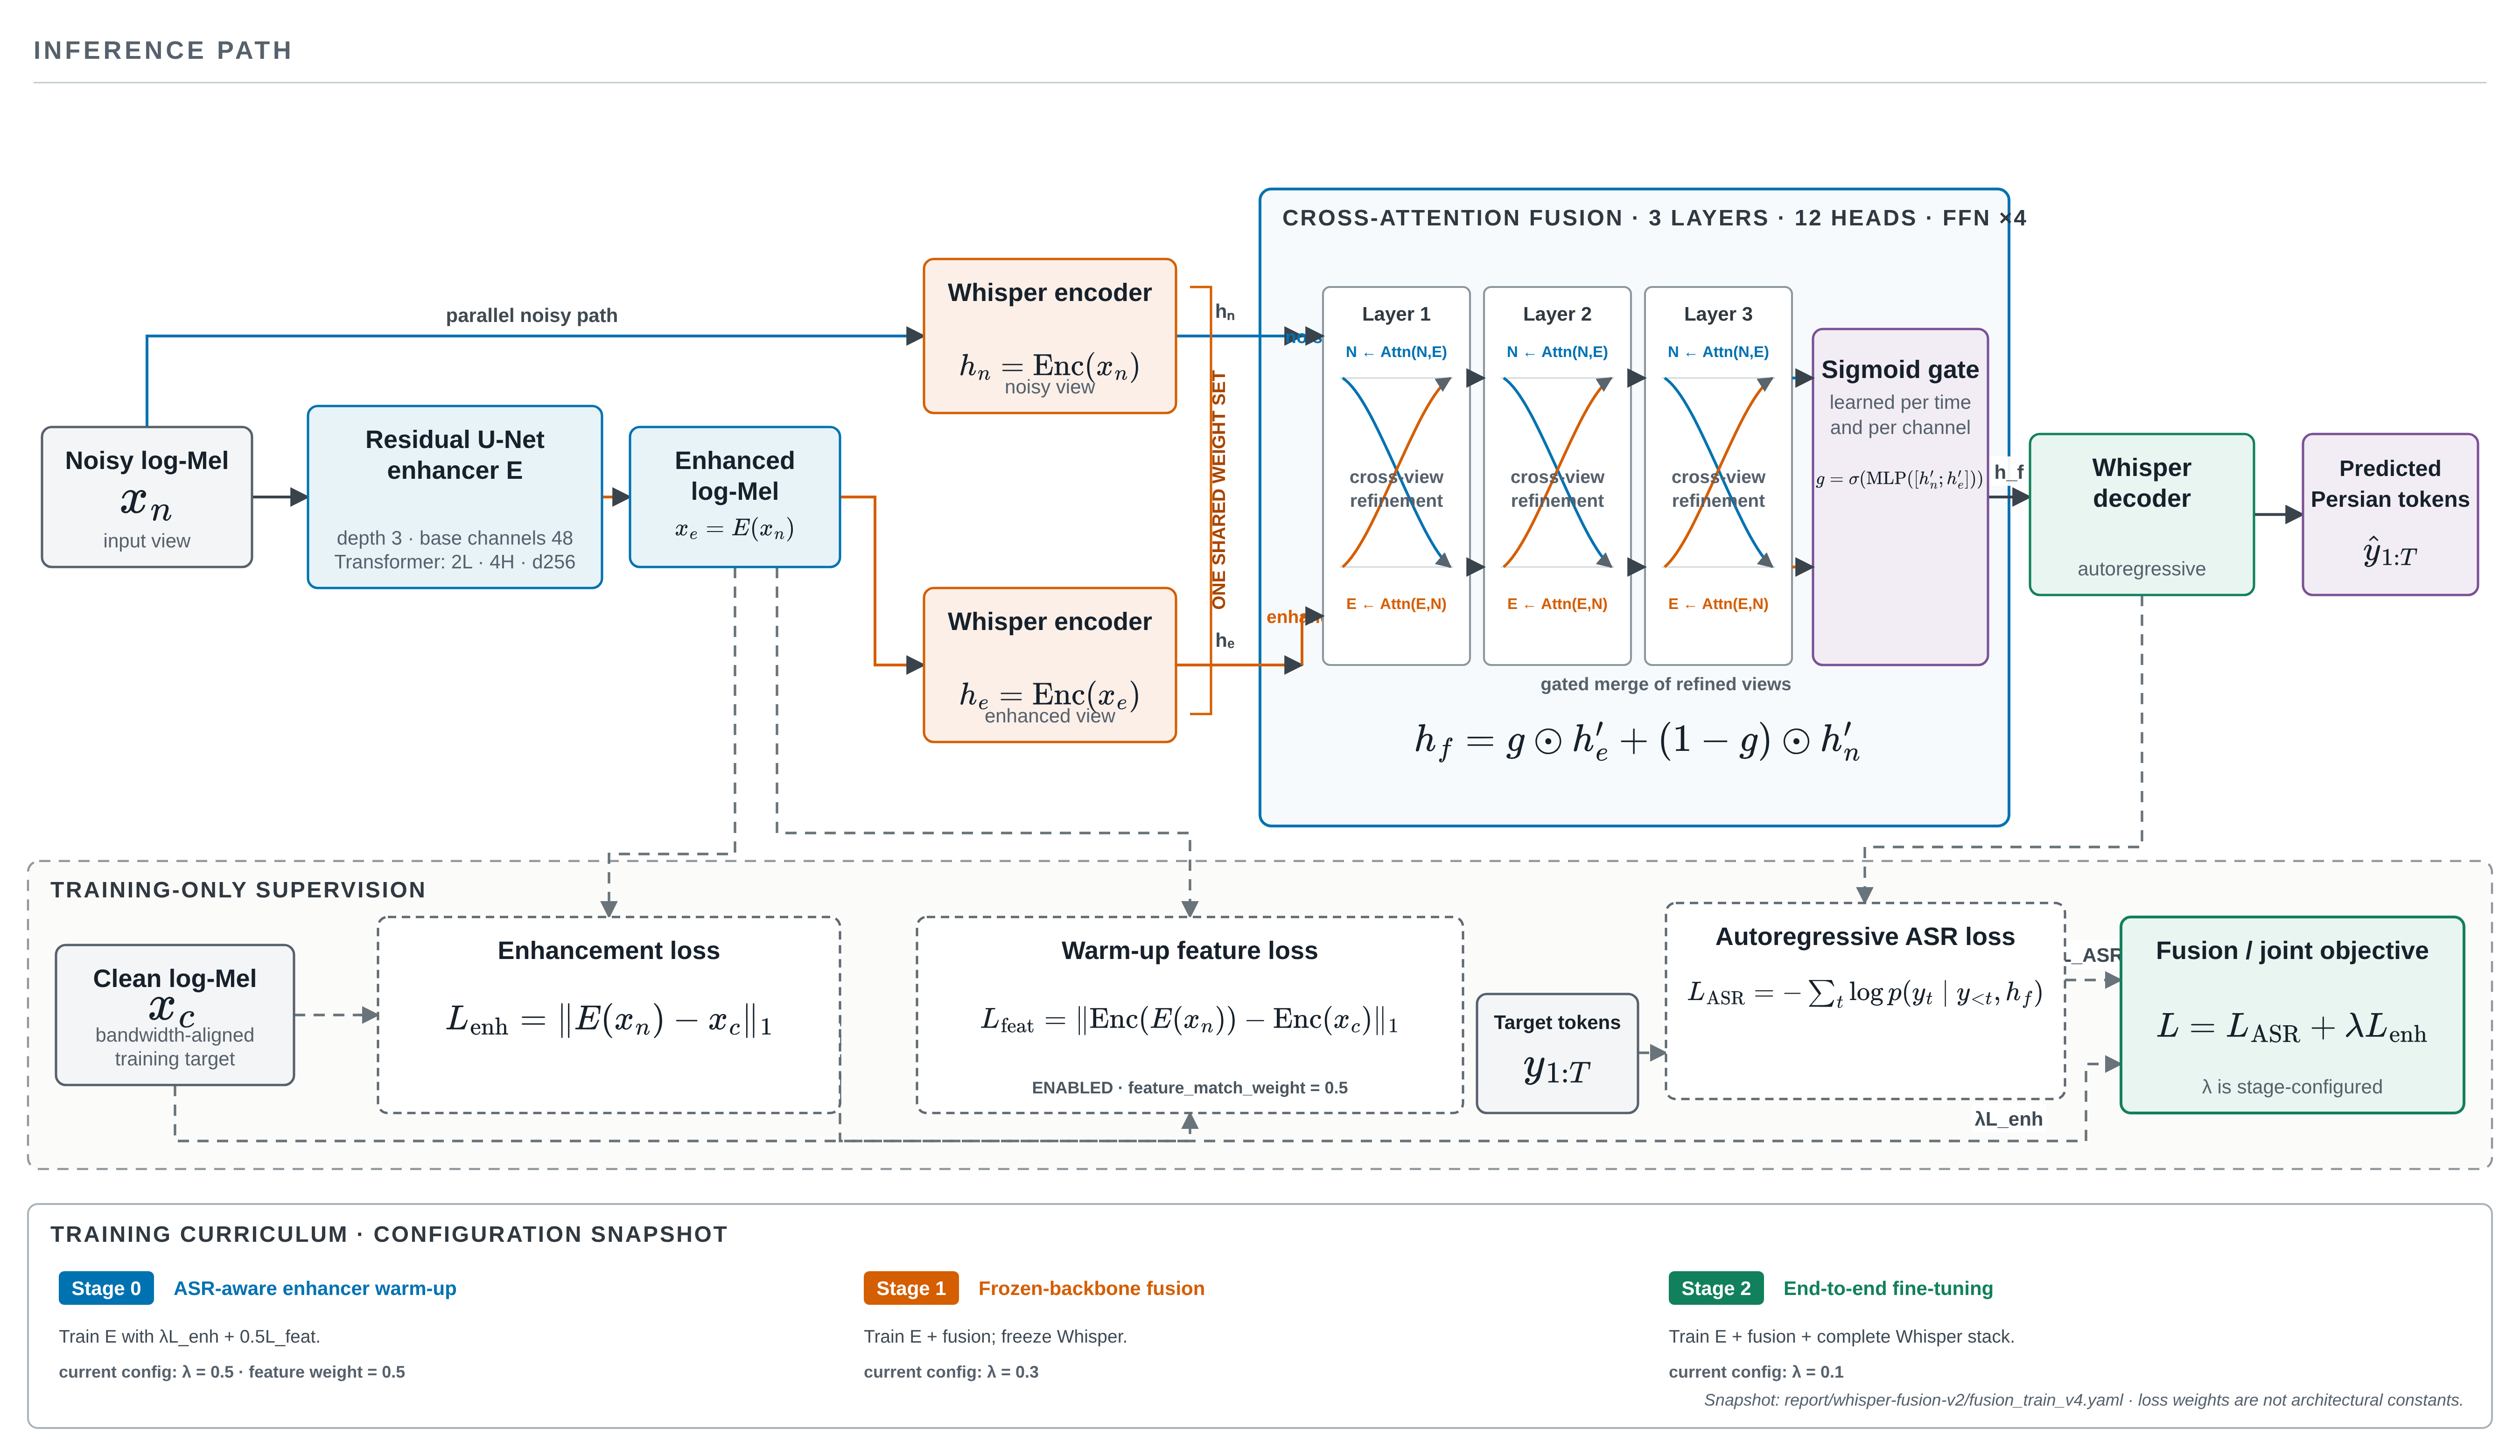
\includegraphics[width=\linewidth,height=0.38\textheight,keepaspectratio]{figs/fusion-model-architecture.png}
\شرح{معماری مدل همجوشی دوجریانه}
\برچسب{شکل:معماری-همجوشی-دوجریانه}
\پایان{شکل}

\زیرقسمت{بهساز در حوزهٔ لاگ-مل}

بهساز $E$ به‌جای بازسازی موج صوتی، مستقیماً بازنمایی ورودی ویسپر را پردازش می‌کند. لاگ-مل ورودی تخریب‌شده را با $\mathbf{M}_n\in\mathbb{R}^{B\times80\times T}$ نشان می‌دهیم که در آن $B$ اندازهٔ دسته، $80$ تعداد باندهای مل و $T$ تعداد قاب‌های زمانی است. خروجی به‌صورت باقیمانده تعریف می‌شود:

\begin{equation}
\mathbf{M}_e=\mathbf{M}_n+E(\mathbf{M}_n).
\end{equation}

در این تعریف، $E(\mathbf{M}_n)$ میزان اصلاح ورودی را تولید می‌کند و مقدار نزدیک صفر، ورودی را تقریباً بدون تغییر نگه می‌دارد.

$E$ یک U-Net دوبعدی باقیمانده با سه سطح و $48$ کانال پایه است \مرجع{ronneberger2015unet}. هر بلوک از کانولوشن $3\times3$، نرمال‌سازی گروهی و تابع فعال‌سازی \کد{GELU} تشکیل شده است و اتصال‌های پرشی اطلاعات زمان-فرکانس را از مسیر پایین‌رو به مسیر بالارو منتقل می‌کنند. در بخش میانی شبکه نیز یک رمزگذار ترنسفورمری دولایه با چهار سر توجه و بُعد $256$ برای مدل‌سازی وابستگی‌های زمانی بلندتر به کار رفته است \مرجع{vaswani2017attention}.

لایهٔ خروجی U-Net و تصویر باقیمانده گلوگاه با صفر مقداردهی اولیه می‌شوند. در آغاز آموزش، $E(\mathbf{M}_n)=0$ و در نتیجه $\mathbf{M}_e=\mathbf{M}_n$ است. به این ترتیب، مدل کار خود را از نگاشت همانی آغاز می‌کند و در گام‌های نخست ویژگی‌هایی با مقیاس نامعمول به ویسپر نمی‌دهد.

هدف بازسازی، خطای $L_1$ میان لاگ-مل بهسازی‌شده و هدف پاکِ هم‌پهنای‌باند $\mathbf{M}_c$ است:

\begin{equation}
\mathcal{L}_{\mathrm{enh}}=\left\|\mathbf{M}_e-\mathbf{M}_c\right\|_1.
\end{equation}

در این رابطه، $\mathbf{M}_c$ لاگ-مل هدف پاکِ هم‌پهنای‌باند است. چون هدف در همان حوزه ورودی ویسپر تعریف می‌شود، نیازی به بازسازی موج یا فاز نیست. زیان بهسازی در مراحل اصلی نقشی کمکی دارد و آنتروپی متقاطع بازشناسی هدف غالب آموزش می‌شود؛ کاهش خطای بهسازی لزوماً نرخ خطای بازشناسی را کاهش نمی‌دهد \مرجع{iwamoto2022bad}.

\زیرقسمت{رمزگذاری مشترک و همجوشی}

هر دو بازنما سپس با یک رمزگذار مشترک ویسپر پردازش می‌شوند:

\begin{equation}
\mathbf{H}_n=\mathrm{Enc}_{\theta}(\mathbf{M}_n),\qquad
\mathbf{H}_e=\mathrm{Enc}_{\theta}(\mathbf{M}_e).
\end{equation}

اشتراک وزن‌ها دو بازنما را در یک فضای بازنمایی مشترک قرار می‌دهد و از افزودن نسخه دوم پارامترهای ویسپر جلوگیری می‌کند، هرچند رمزگذار برای هر نمونه دو بار اجرا می‌شود.


همجوشی پس از رمزگذار و در سه لایه انجام می‌شود. هر لایه شامل توجه متقاطع دوسویه با $12$ سر و یک شبکهٔ پیش‌خور باقیمانده است که بُعد میانی آن چهار برابر بُعد نهان است. توجه متقاطع پیش از اعمال دروازه میان دو جریان اطلاعات مبادله می‌کند.

خروجی‌های پالایش‌شده را با $\mathbf{H}'_n$ و $\mathbf{H}'_e$ نشان می‌دهیم. پس از تبادل اطلاعات، یک دروازه برای هر گام زمانی و هر مؤلفه نهان ساخته می‌شود:

\begin{equation}
\mathbf{g}=\sigma\!\left(W_2\,\mathrm{GELU}\!\left(W_1[\mathbf{H}'_n;\mathbf{H}'_e]\right)\right),
\qquad
\mathbf{H}_f=\mathbf{g}\odot\mathbf{H}'_e+(1-\mathbf{g})\odot\mathbf{H}'_n.
\end{equation}

عملگر $[\,;\,]$ الحاق، $\sigma$ سیگموید و $\odot$ ضرب عضو‌به‌عضو است. مقدار نزدیک یک در $\mathbf{g}$ سهم نمای بهسازی‌شده و مقدار نزدیک صفر سهم نمای اصلی را افزایش می‌دهد؛ این وزن برای هر گام زمانی و مؤلفهٔ نهان جداگانه محاسبه می‌شود.


خروجی لایه‌های توجه و پیش‌خور با صفر مقداردهی اولیه می‌شود. ورودی تابع سیگموید دروازه نیز در ابتدا صفر است؛ ازاین‌رو، هر بازنما در آغاز وزن $0.5$ دارد. بازنمایی نهایی $\mathbf{H}_f$ به رمزگشای بدون‌تغییر ویسپر داده می‌شود. برخلاف کارهای همجوشی پیشین، نقطهٔ آغاز این آزمایش ویسپری است که پیش‌تر با همان خانواده تخریب‌های مخابراتی آموزش دیده است \مرجع{fujimoto2019onepass,zhu2022joint,yang2023fathubert,hu2024wav2code,wang2024bridge}.

\زیرقسمت{برنامه آموزش سه‌مرحله‌ای}

آموزش هم‌زمان بخش‌های جدید شبکه و ویسپر از همان ابتدای کار می‌تواند وزن‌های ازپیش‌آموخته مدل را پیش از شکل‌گیری مناسب بخش‌های تازه تغییر دهد. از سوی دیگر، اگر بهساز پس از آموزش بازسازی ثابت بماند، فرصتی برای سازگارشدن با هدف بازشناسی گفتار پیدا نمی‌کند. به همین دلیل، آموزش به‌صورت مرحله‌ای طراحی شد تا ابتدا بهساز آموزش ببیند و سپس اجزای مدل به‌تدریج برای آموزش انتهابه‌انتها آزاد شوند.

در مدل همجوشی نیز مانند آزمایش‌های پیشین، ویسپر-کوچک به‌عنوان ستون فقرات بازشناسی استفاده شد. مراحل آموزش و سقف تعداد گام‌ها به‌صورت زیر در نظر گرفته شدند:

\شروع{فقرات}
\فقره \مهم{گرم‌کردن بهساز:} فقط $E$ و حداکثر تا $20{,}000$ گام آموزش دید. علاوه بر $\mathcal{L}_{\mathrm{enh}}$، فاصلهٔ $L_1$ میان ویژگی‌های رمزگذار برای نمای بهسازی‌شده و هدف پاک نیز محاسبه شد. با نمایش این مؤلفه به‌صورت $\mathcal{L}_{\mathrm{feat}}$، تابع هدف برابر $0.5\mathcal{L}_{\mathrm{enh}}+0.5\mathcal{L}_{\mathrm{feat}}$ بود. مؤلفهٔ دوم خروجی بهساز را از دید رمزگذار ویسپر نیز به هدف پاک نزدیک کرد. در این مرحله، صوت‌های تخریب‌شده همراه با جفت پاک متناظر آن‌ها استفاده شدند؛
\فقره \مهم{آموزش همجوشی با ستون فقرات ثابت:} بهساز و بلوک همجوشی حداکثر تا $30{,}000$ گام با تابع هدف $\mathcal{L}_{\mathrm{ASR}}+0.3\mathcal{L}_{\mathrm{enh}}$ آموزش دیدند. وزن‌های ویسپر در این مرحله ثابت بودند تا بخش‌های تازه بدون تغییر زودهنگام ستون فقرات، بازنمایی مناسب برای بازشناس موجود را بیاموزند. در این مرحله نیز صوت‌های تخریب‌شده، جفت پاک متناظر و رونوشت متنی آن‌ها استفاده شدند؛ و
\فقره \مهم{آموزش مشترک انتهابه‌انتها:} در مرحله نهایی، ماژول‌های بهساز، همجوشی و ویسپر حداکثر تا $120{,}000$ گام با هم آموزش دیدند. تابع هدف $\mathcal{L}_{\mathrm{ASR}}+0.1\mathcal{L}_{\mathrm{enh}}$ بود؛ کاهش وزن زیان بهسازی، اولویت بیشتری به بازشناسی داد. نرخ یادگیری بخش جلویی $10^{-4}$ و نرخ یادگیری ویسپر $5\times10^{-6}$ بود تا ستون فقرات به‌آرامی با بخش‌های تازه سازگار شود. در این مرحله، کل داده‌های آموزشی شامل داده‌های پاک، تخریب‌شده و نمونه‌های بلند، استفاده شدند.
\پایان{فقرات}

در دو مرحلهٔ پایانی، مدل در فاصله‌های منظم روی بخش اعتبارسنجی تخریب‌شده ارزیابی شد و بهترین نسخهٔ ذخیره‌شدهٔ مدل بر اساس کمترین \lr{WER} انتخاب شد. نسخه‌های مدل در طول آموزش و در پایان هر مرحله ذخیره شدند تا در صورت ادامهٔ اجرا، نیازی به تکرار مراحل تکمیل‌شده نباشد.


داده‌های پاک در مرحله نهایی حضور داشتند، اما وارد مراحل ویژه یادگیری بهسازی نشدند. در نمونه پاک، ورودی و هدف بهسازی یکسان بودند؛ بنابراین، بهساز به حفظ نگاشت همانی تشویق شد. این نمونه‌ها هم‌زمان ویسپر را روی گفتار معمولی ریزتنظیم کردند و خطر پسرفت در دامنه پاک را کاهش دادند. در مقابل، داده‌های تخریب‌شده هر سه مرحله را هدایت کردند، زیرا فقط آن‌ها جفت پاک-تخریب‌شده و هدفی معنادار برای $\mathcal{L}_{\mathrm{enh}}$ داشتند.


\زیرقسمت{پروتکل تحلیل دروازه}

مقایسهٔ \lr{WER} و \lr{CER} عملکرد نهایی سامانه را نشان می‌دهد، اما مشخص نمی‌کند مدل تا چه اندازه به هر یک از دو نما متکی است. برای بررسی این موضوع، هنگام رمزگشایی مقدار دروازهٔ آموخته‌شده $\mathbf{g}\in[0,1]^{T\times D}$ برای هر نمونه ثبت شد. با میانگین‌گیری از $\mathbf{g}$ روی گام‌های زمانی و ابعاد نهان، سهم نمای بهسازی‌شده برای هر کلیپ محاسبه شد و سپس میانگین و میانهٔ آن در کل مجموعهٔ ارزیابی گزارش شد. سهم نمای اصلی نیز برابر با یک منهای سهم نمای بهسازی‌شده در نظر گرفته شد.

از آنجا که دو جریان پیش از اعمال دروازه از طریق توجه متقاطع با یکدیگر اطلاعات مبادله می‌کنند، این میانگین را نمی‌توان مستقیماً به سهم مستقل هر جریان تعبیر کرد و تغییرات موضعی وزن‌ها را نیز نشان نمی‌دهد. بنابراین، این آمار تنها برای بررسی گرایش کلی دروازه به یکی از دو نما استفاده می‌شود.



\قسمت{افزایش مقیاس داده با صوت بلند ایران‌صدا}

در این آزمایش، معماری ویسپر-کوچک و ترکیب چندشرایطی ثابت ماند و پیکره‌ای شبه‌برچسب‌خورده از کتاب‌های صوتی فارسی به داده‌های آموزش افزوده شد. این مقایسه اثر افزودن داده بیشتر از دامنه‌ای تازه را بدون تغییر معماری می‌سنجد. کتاب صوتی از نظر سبک و کانال با تماس تفاوت دارد؛ ازاین‌رو، نتایج آن برای مجموعه‌های عمومی و مخابراتی جداگانه گزارش می‌شوند \مرجع{kahn2020selftraining,likhomanenko2021slimipl,bhogale2024pseudolabel}.

\شروع{شکل}[htbp]
\centering
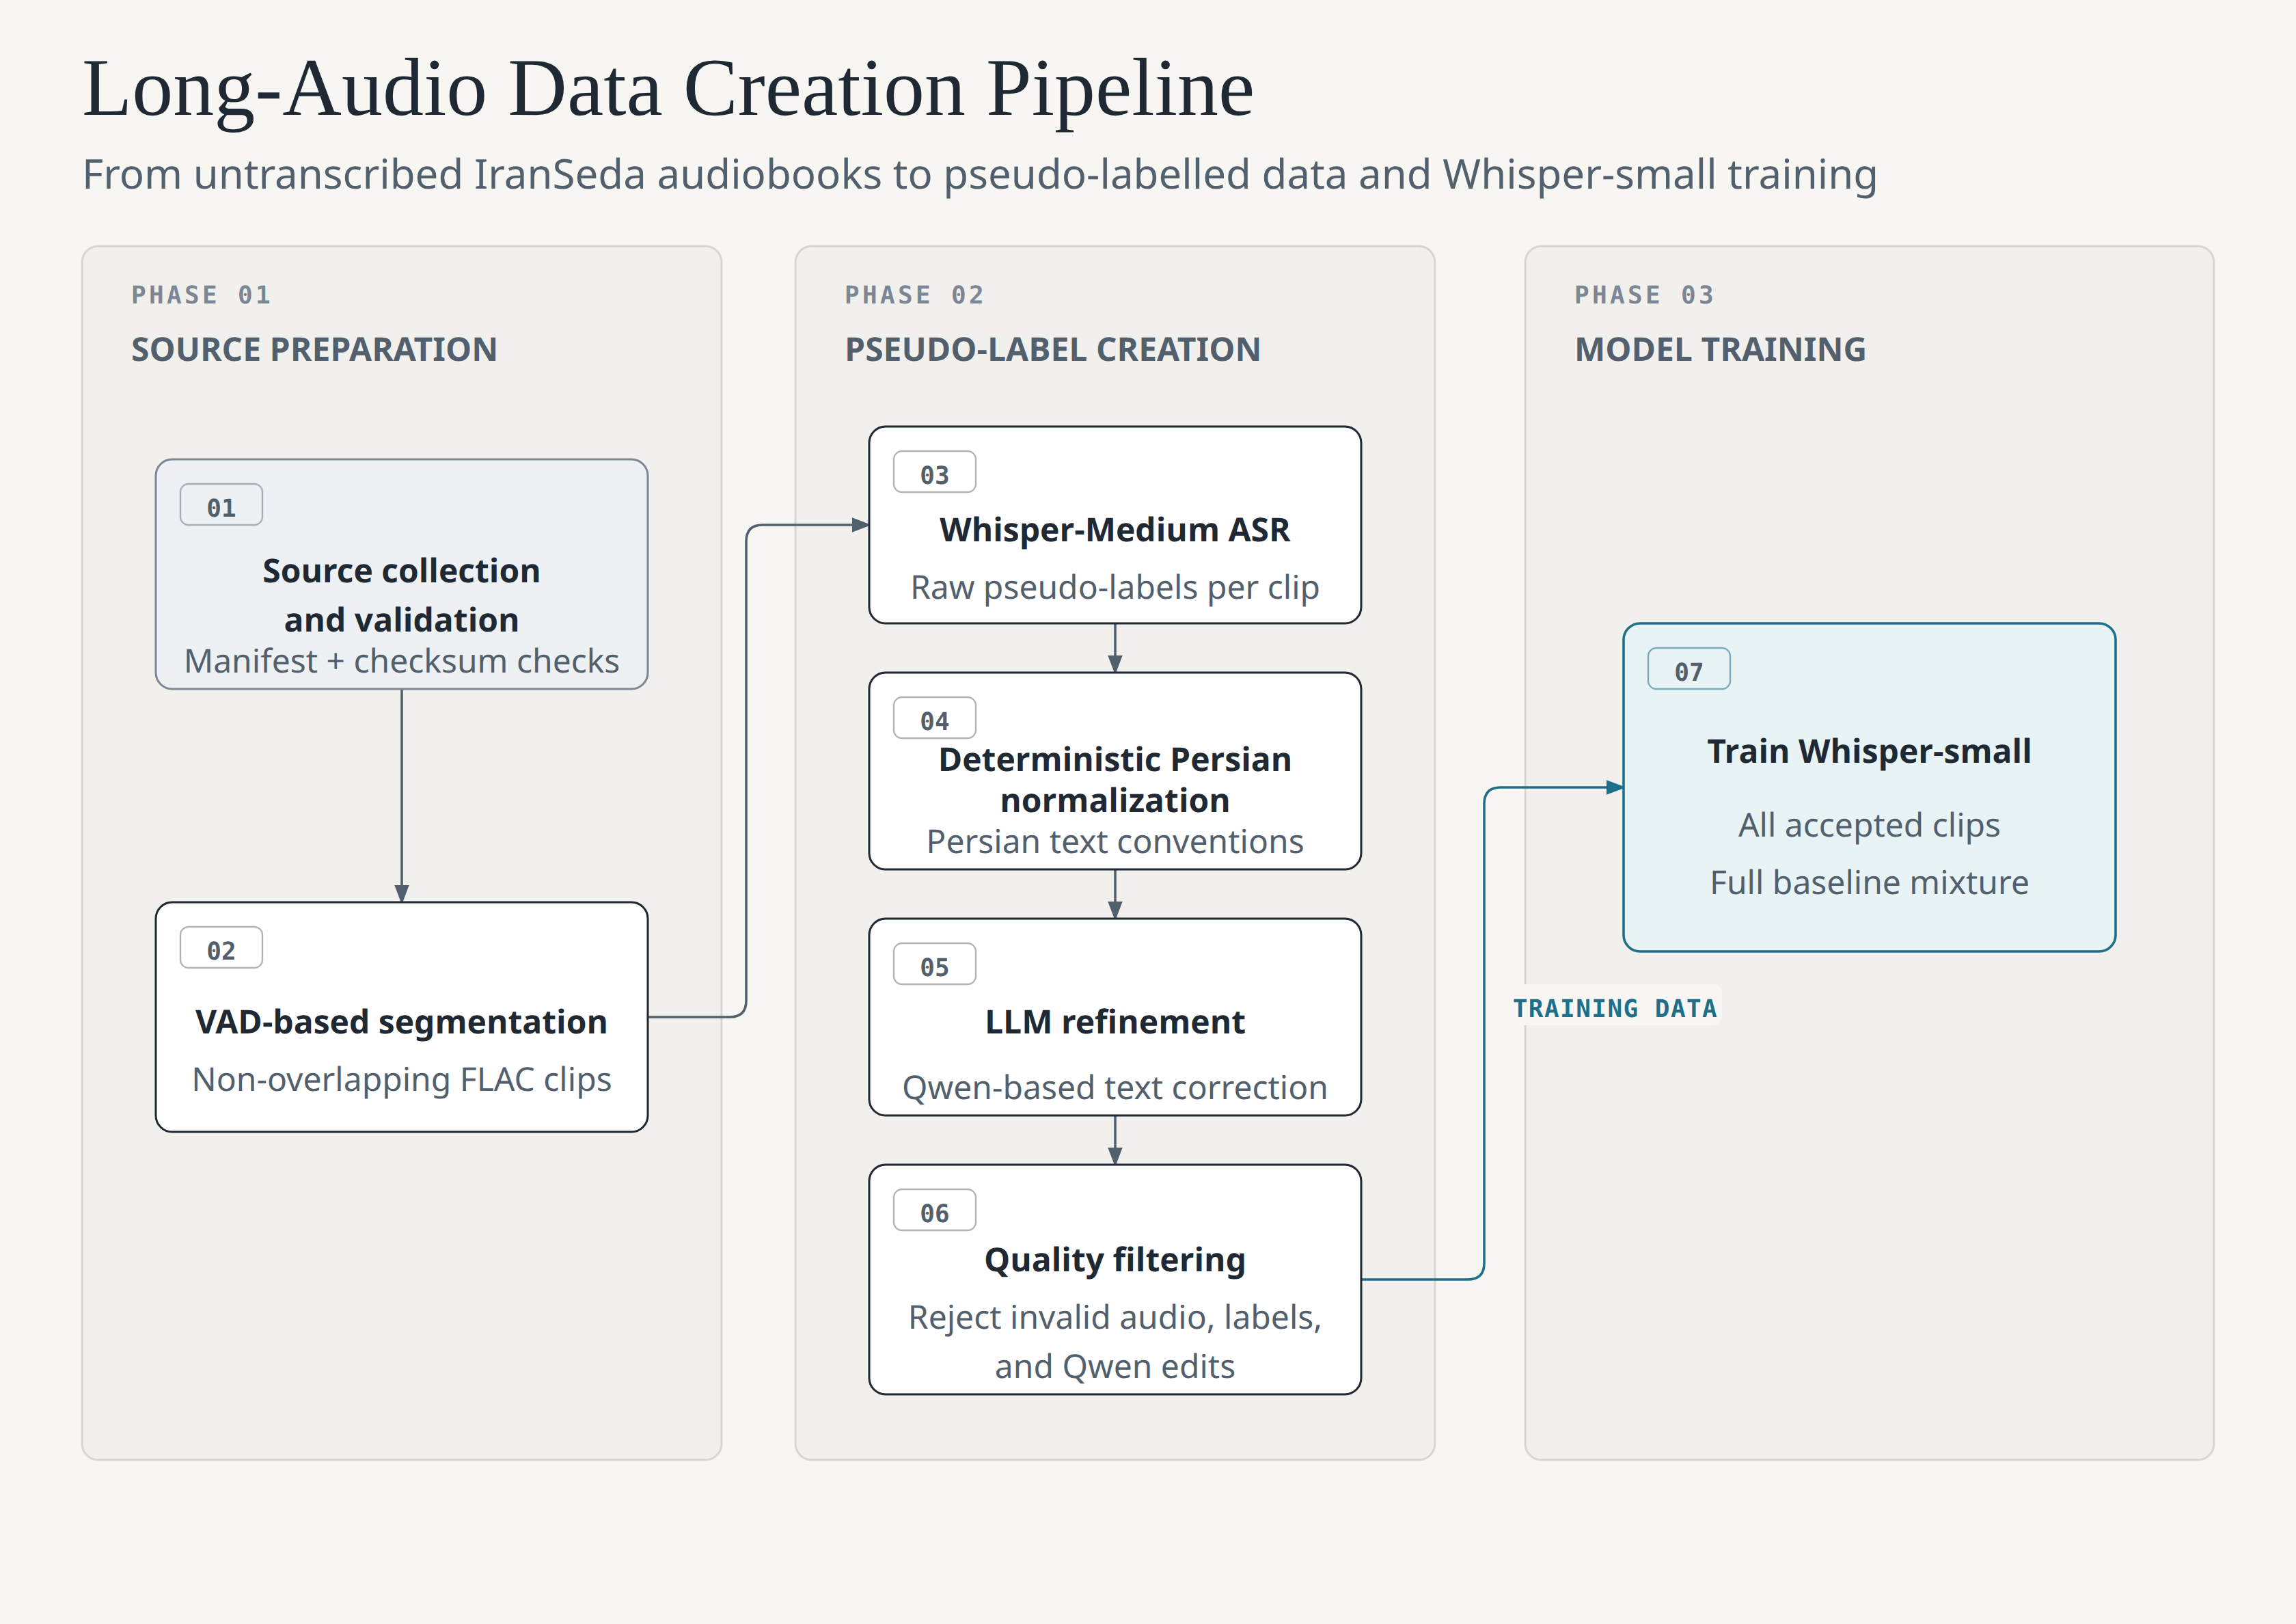
\includegraphics[width=\linewidth,height=0.62\textheight,keepaspectratio]{figs/long-audio-data-creation-pipeline.png}
\شرح{خط لوله سرتاسری ساخت داده شبه‌برچسب‌خورده از صوت بلند ایران‌صدا. پس از گردآوری و اعتبارسنجی منبع، قطعه‌ها رونویسی، نرمال‌سازی، اصلاح و پالایش شدند و همه نمونه‌های پذیرفته‌شده برای آموزش ویسپر-کوچک به ترکیب کامل داده‌های خط مبنا افزوده شدند.}
\برچسب{شکل:خط-لوله-ساخت-داده-صوت-بلند}
\پایان{شکل}

\زیرقسمت{گردآوری، اعتبارسنجی و انتخاب منابع}

برای این آزمایش، کتاب‌های صوتی از بخش عمومی وب‌گاه ایران‌صدا گردآوری شدند. این فرایند دو مرحله داشت: استخراج فراداده و دریافت صوت. عنوان، نویسنده، گوینده، مدت، شناسهٔ منبع، نشانی صفحه و پیوند فایل صوتی در رکوردهای \کد{JSONL} ذخیره شدند تا هر فایل و خروجی‌های مشتق‌شده از آن قابل ردیابی باشند.

فایل‌های صوتی فقط از پیوندهای ثبت‌شده دریافت شدند و موارد تهی، نامعتبر یا رمزگشایی‌ناپذیر کنار گذاشته شدند. درهم‌سازی \کد{SHA-256}، مسیر محلی و اطلاعات منبع نیز در سیاههٔ دریافت ثبت شد تا بتوان فایل‌ها را وارسی و مراحل را دوباره اجرا کرد.

در مجموع $3{,}777$ کتاب صوتی، معادل حدود $6{,}300$ ساعت صوت خام، دریافت شد. با توجه به توان محاسباتی موجود، $250$ ساعت از این مجموعه برای آماده‌سازی نهایی و آزمایش انتخاب شد. انتخاب در سطح منبع انجام گرفت تا قطعه‌های یک کتاب به‌صورت پراکنده وارد یا حذف نشوند.

پیش از قطعه‌بندی، وجود فایل، تطابق درهم‌سازی و امکان رمزگشایی صوت بررسی شد. فایل خام دست‌نخورده باقی ماند و خروجی هر مرحله با شناسه منبع اصلی ذخیره شد.

\زیرقسمت{قطعه‌بندی مبتنی بر فعالیت گفتاری}

ویسپر ورودی‌هایی در حدود $30$ ثانیه را پردازش می‌کند، درحالی‌که فایل هر کتاب ممکن است چند ساعت طول داشته باشد. فایل‌ها ابتدا با \کد{FFmpeg} به صوت تک‌کاناله با نرخ $16$ کیلوهرتز تبدیل و سپس با مدل تشخیص گفتار سیلرووَد\پاورقی{SilerVAD} قطعه‌بندی شدند. آستانهٔ VAD برابر $0.5$ بود و استنتاج روی GPU انجام شد.

طول هدف قطعه‌ها $20$ ثانیه و بازهٔ ترجیحی $15$ تا $25$ ثانیه بود. مرزها تا حد ممکن روی سکوت یا افت انرژی قرار گرفتند و در نبود مرز مناسب، سقف سخت $28$ ثانیه اعمال شد. قطعه‌های طبیعی کوتاه با دست‌کم دو ثانیه گفتار حفظ شدند و هیچ دو قطعه‌ای هم‌پوشانی نداشتند. خروجی قطعه‌بند برای هر قطعه یک فایل صوتی تک‌کاناله، $16$ کیلوهرتزی و بدون اتلاف بود. شناسه قطعه از شناسه منبع و شماره‌ای ترتیبی و پایدار ساخته شد. 

\زیرقسمت{شبه‌برچسب‌گذاری و نرمال‌سازی قطعی}

برای تولید شبه‌برچسب، هر قطعه با ویسپر-متوسطِ ریزتنظیم شده رونویسی شد. این مدل پیش‌تر با مجموعه داده‌های چندشرایطی پروژه، شامل داده‌های اصلی و نسخه‌های تخریب‌شده، آموزش دیده شد. آموزش در یک دوره با نرخ یادگیری $10^{-5}$، اندازهٔ دسته $2$ و انباشت گرادیان در $8$ گام انجام شد. هنگام رونویسی نیز مدل روی زبان فارسی و وظیفهٔ \کد{transcribe} تنظیم شد.
خروجی ویسپر ابتدا به‌صورت خام ذخیره و سپس با همان نرمال‌ساز فارسی مورد استفاده در سایر داده‌ها پردازش شد. هر دو نسخه خام و نرمال‌شده نگهداری شدند و قطعه‌هایی که رونویسی معتبر نداشتند کنار گذاشته شدند. عملکرد این مدل روی مجموعه‌های آزمون نیز به‌عنوان یک ارزیابی تکمیلی گزارش شد.



\زیرقسمت{اصلاح محافظه‌کارانه با مدل زبانی}

نرمال‌سازی متنی بسیاری از تفاوت‌های ظاهری را برطرف می‌کند، اما بعضی خطاها تنها با توجه به بافت جمله قابل تشخیص‌اند. برای اصلاح محدود این موارد، از مدل کوانتیزه‌شده \کد{cyankiwi/Qwen3.6-27B-AWQ-INT4} استفاده شد. این مدل فقط متن را دریافت می‌کرد و مجاز بود خطاهای آشکار را اصلاح کند؛ بازنویسی متن، افزودن محتوا یا کامل‌کردن جمله‌های ناقص مجاز نبود.

برای درک بهتر بافت\پاورقی{Context}، در صورت وجود تا سه قطعه قبل و سه قطعه بعد از همان کتاب نیز در اختیار مدل قرار گرفت. بافت پیشین از نسخه‌های اصلاح‌شده و پذیرفته‌شدهٔ قطعه‌های قبلی و بافت پسین از خروجی نرمال‌شدهٔ ویسپر تشکیل شد. عنوان و توضیح کتاب نیز، در صورت وجود، به مدل ارائه شد. تولید با دمای صفر انجام شد تا تغییرات تا حد ممکن محدود و تکرارپذیر باشند. شکل~\رجوع{شکل:پرامپت-اصلاح-رونویسی} قالب پرامپت استفاده‌شده را نشان می‌دهد.

\شروع{شکل}[htbp]
\centering
\fbox{%
\begin{minipage}{0.94\linewidth}
\begin{latin}
\scriptsize
\ttfamily
\setlength{\parindent}{0pt}
\raggedright

Refine one Persian ASR segment conservatively. Modify only the TARGET WHISPER TEXT.

\medskip
Allowed corrections:

- Persian orthography and spelling

- spacing and نیم‌فاصله

- punctuation when clearly justified

- obvious ASR word substitutions when the intended spoken word is strongly supported by the target and context

\medskip
Rules:

- Preserve the meaning and wording of the spoken target as closely as possible.

- Use surrounding context only to disambiguate the target.

- Never copy words or phrases from the context into the target unless they clearly correct an ASR error already present in the target.

- Never complete an incomplete phrase at a segment boundary.

- Never add, infer, summarize, or rewrite speech that is not present in the target.

- Do not remove valid spoken words merely to improve fluency.

- Preserve every numeric token exactly as written, including digits, signs, separators, and formatting.

- When a correction is not sufficiently certain, keep the original text and set uncertain=true.

- Set uncertain=false only when all applied corrections are high-confidence.

- Return only the required JSON object with no explanation or Markdown.

\medskip
[AUDIOBOOK TITLE]

\textless audiobook title or (omitted)\textgreater

\medskip
[AUDIOBOOK DESCRIPTION]

\textless audiobook description or (omitted)\textgreater

\medskip
[REFINED PRECEDING CONTEXT]

\textless up to three previously accepted refined segments or (none)\textgreater

\medskip
[TARGET WHISPER TEXT]

\textless normalized target transcription\textgreater

\medskip
[FOLLOWING WHISPER CONTEXT]

\textless up to three following normalized Whisper segments or (none)\textgreater

\end{latin}
\end{minipage}%
}
\شرح{قالب پرامپت استفاده‌شده برای اصلاح محافظه‌کارانهٔ هر قطعه صوتی شبه‌‌برچسب‌خورده. عبارت‌های داخل نشانه‌های زاویه‌دار در زمان اجرا با فراداده و متن قطعه‌های همان کتاب جایگزین می‌شدند.}
\برچسب{شکل:پرامپت-اصلاح-رونویسی}
\پایان{شکل}

در پایان، خروجی‌هایی که تهی، نامطمئن یا غیرفارسی بودند، اعداد را تغییر می‌دادند یا نسبت به متن اولیه تغییر زیادی داشتند، کنار گذاشته شدند. برای مورد آخر، آستانه فاصله ویرایشی نرمال‌شده برابر با $0.55$ در نظر گرفته شد. متن اولیه ویسپر نیز در همه مراحل حفظ شد و نسخه اصلاح‌شده به‌صورت جداگانه ذخیره شد.

\زیرقسمت{پالایش کیفیت و تفکیک داده}

در پالایش داده، تنها قطعه‌هایی نگه داشته شدند که مدت آن‌ها در بازهٔ تعیین‌شده قرار داشت و شامل مقدار کافی گفتار و رونویسی فارسیِ معتبر بودند. خروجی‌های نامطمئن مدل زبانی، مواردی که در آن‌ها اعداد تغییر کرده بودند و قطعه‌های صوتی تکراری یا هم‌پوشان نیز کنار گذاشته شدند.

در مجموع $44{,}820$ قطعه بررسی شد که از میان آن‌ها $39{,}454$ قطعه از $136$ فایل کتاب صوتی پذیرفته و $5{,}366$ قطعه رد شدند. علاوه بر این، $40$ شکست عملیاتی نیز به‌صورت جداگانه ثبت شد. دادهٔ پذیرفته‌شده در نهایت شامل $218.564$ ساعت صوت بود. بنابراین، «زیرمجموعهٔ $250$ ساعته» به دادهٔ انتخاب‌شده پیش از پالایش اشاره دارد و حجم نهایی پیکرهٔ آموزشی $218.564$ ساعت بود.

تقسیم داده آموزش و اعتبارسنجی در سطح کتاب انجام شد تا قطعه‌های یک کتاب میان آموزش و اعتبارسنجی پخش نشوند. همه قطعه‌های متعلق به یک کتاب، حتی اگر از چند فایل صوتی استخراج شده بودند، در یک بخش قرار گرفتند. این تقسیم به‌صورت ثابت و مستقل از ترتیب فایل‌ها انجام شد. به این ترتیب، بخش‌های نزدیک یک کتاب و تا حد امکان صدای یک راوی میان آموزش و اعتبارسنجی مشترک نبود. مجموعه‌های آزمون نیز مستقل باقی ماندند و هیچ‌یک از فایل‌های شبه‌برچسب‌خورده به آن‌ها اضافه نشد.


\زیرقسمت{آزمایش نهایی افزایش مقیاس داده}

مدل مرجع این آزمایش همان ویسپر-کوچک چندشرایطی بود که با داده معمولی فارسی، گونه‌های بلند و دادهٔ مصنوعاً تخریب‌شده آموزش دیده بود. مدل جدید همین ترکیب را حفظ کرد و داده‌های پذیرفته‌شدهٔ کتاب صوتی را به آن افزود. هر دو اجرا از از تعداد گام آموزشی، نرخ یادگیری $10^{-5}$، اندازهٔ دسته $4$ و انباشت گرادیان در $8$ گام استفاده کردند. به این ترتیب، تغییر اصلی میان دو اجرا افزودن داده ایران‌صدا بود.

هر دو مدل با نرمال‌ساز فارسی، پیاده‌سازی WER و CER و قواعد یکسان حذف نمونه‌های نامعتبر روی پنج مجموعه آزمون انسانی ارزیابی شدند. نتایج هم به‌صورت تجمیعی و هم برای هر مجموعه گزارش شدند تا اثر داده تازه بر گفتار عمومی و AGFarsdat تلفنی و \lr{VoIP} جداگانه دیده شود. امتیازدهی دو مدل روی نمونه‌های واجد شرایط مشترک انجام شد.

\قسمت{جمع‌بندی فصل}

این فصل روش‌های اصلی ویسپر-کوچک را در دو محور تعریف کرد. در محور مقاوم‌سازی، ابتدا ویسپر معمولی با ویسپر چندشرایطی و سپس مدل دوجریانه با ویسپر چندشرایطی مقایسه شد. در محور افزایش مقیاس داده، پیکرهٔ $218.564$ ساعتهٔ ایران‌صدا به داده‌های آموزشی مدل چندشرایطی افزوده شد. فست کانفورمر و ویسپر-متوسط نیز به‌عنوان دو آزمایش تکمیلی، به‌ترتیب برای بررسی تأثیر خانوادهٔ معماری و ظرفیت مدل در نظر گرفته شدند. در این مقایسه‌ها، هر تغییر نسبت به مناسب‌ترین خط مبنای پیشین سنجیده شد تا اثر آن به‌صورت مستقل‌تر مشخص شود. فصل بعد نتایج همه این آزمایش‌ها را با پروتکل ارزیابی یکسان گزارش و مقایسه می‌کند.
